\section{Trust Region Motivation}
\begin{frame}{Why Step Size Matters}
\begin{columns}
\begin{column}{0.48\textwidth}
\begin{figure}
\centering
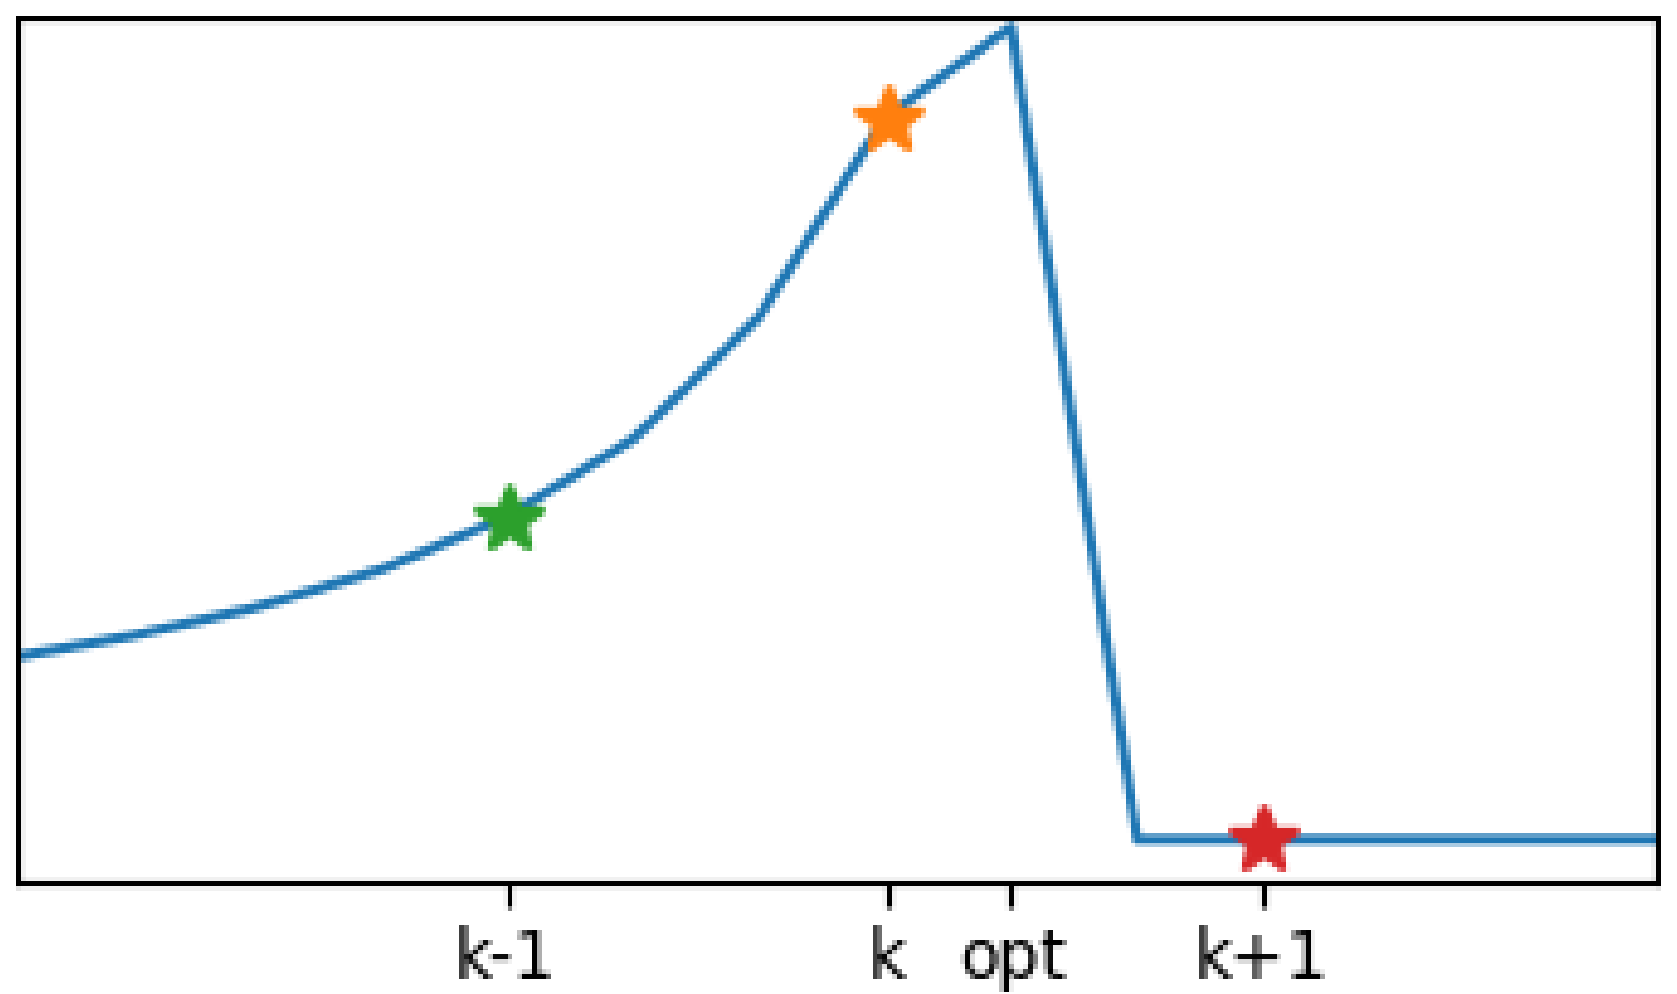
\includegraphics[width=\textwidth,height=0.5\textheight,keepaspectratio]{images/policy-optimization/step_1.png}
\end{figure}
\end{column}
\begin{column}{0.48\textwidth}
\begin{figure}
\centering
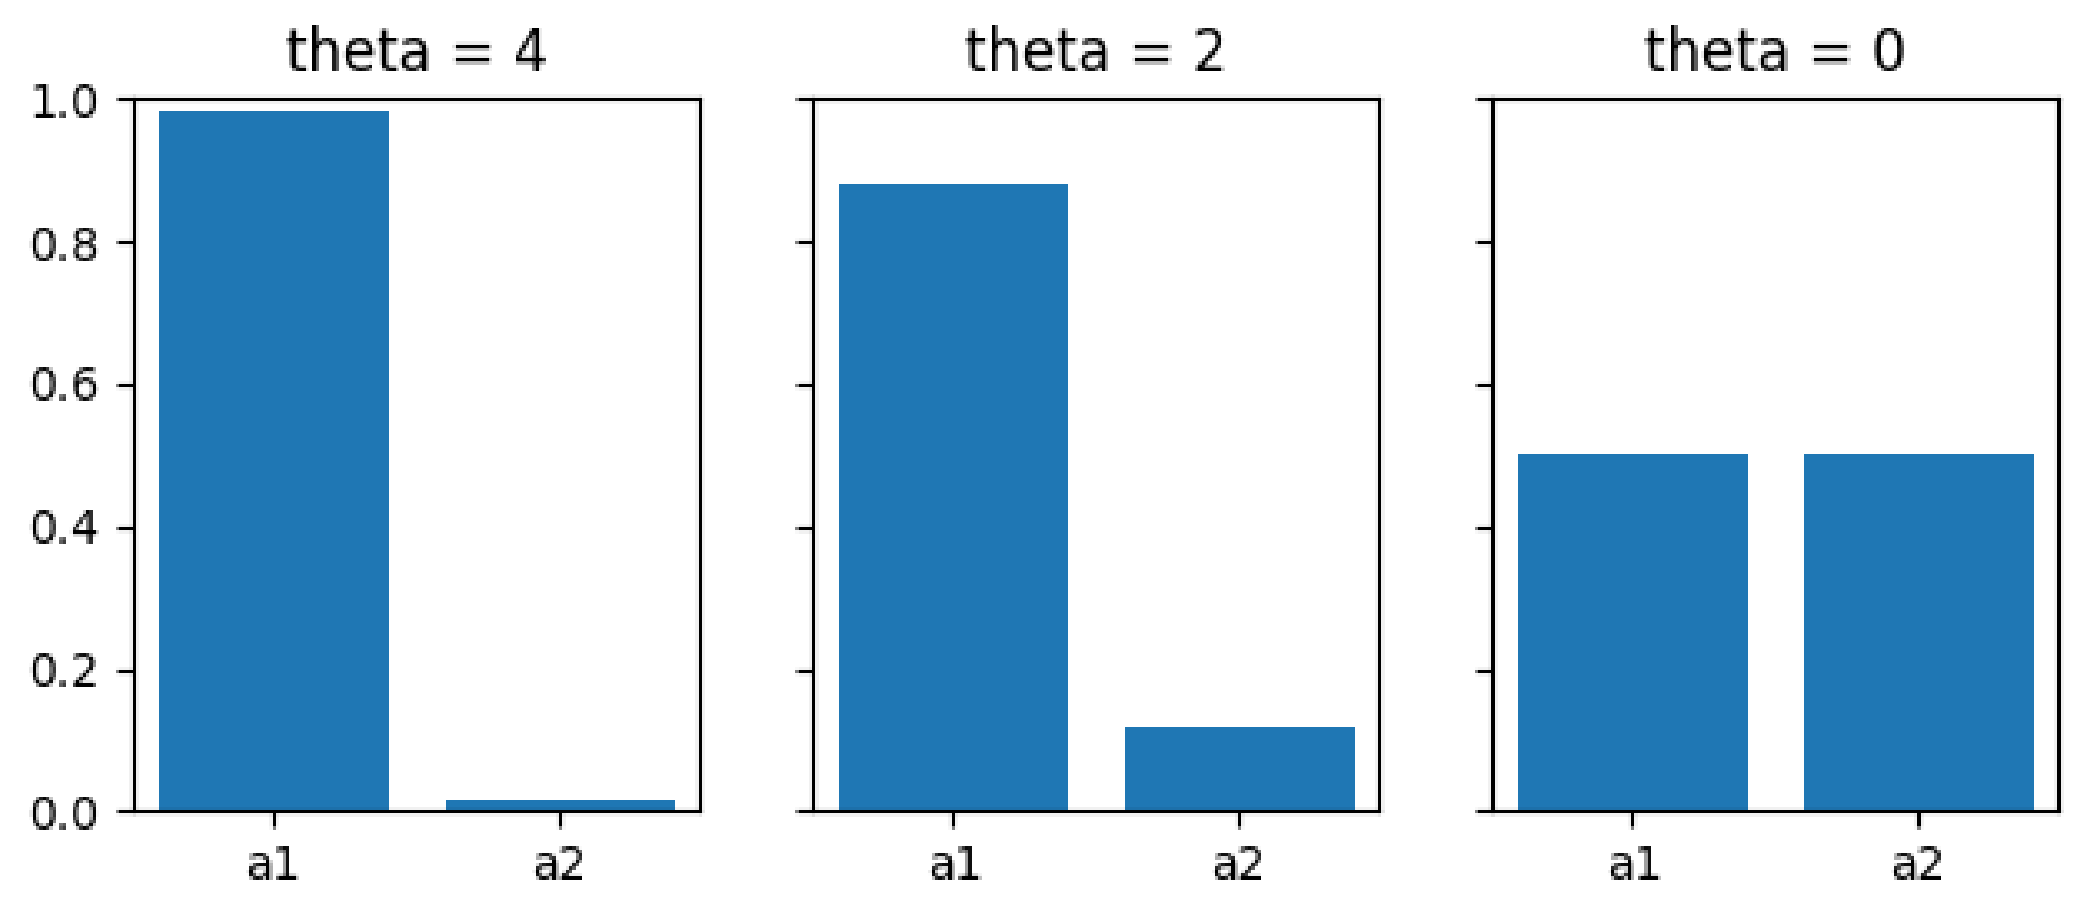
\includegraphics[width=\textwidth,height=0.5\textheight,keepaspectratio]{images/policy-optimization/step_2.png}
\end{figure}
\end{column}
\end{columns}
\vspace{0.5em}
\begin{itemize}
    \item A large gradient step in \emph{parameter space} can cause a catastrophically large shift in \emph{policy space}
    \item Once a policy collapses (e.g., always picks one bad action), the agent collects bad data and the policy is hard to recover
    \item We need to control how much the policy distribution changes, not just how much $\theta$ changes
\end{itemize}
\end{frame}
